This chapter provides a detailed architectural design of Students\&Companies, starting with a high-level overview of the system's design choices and their rationale.
It then explores the component view, illustrating major system modules and their interactions using various UML diagrams.
A deployment view follows, showing how software components distribute across hardware nodes.
Runtime views are then presented through sequence diagrams depicting key system operations.
The chapter concludes with a discussion of chosen architectural styles, patterns and other significant design decisions.

\section{Overview}
Students\&Companies requires an architecture that can efficiently handle the complex interactions between students, companies and universities while ensuring system scalability and data security.
The platform adopts a three-tier client-server architecture, separating presentation, application logic and data management into distinct layers.
This section provides an overview of the application of this architecture to the problem at hand, while a more general discussion of styles and patterns belongs in later sections.

\subsubsection{Presentation Tier}
At the client tier, the web app serves as the user interface, allowing students, companies and universities to access S\&C through their browsers.
The app is designed to be responsive, ensuring accessibility across various devices while maintaining a consistent user experience.

\subsubsection{Application Tier}
The middle tier consists of three server components.

The web server handles incoming client requests, managing user sessions and providing load balancing capabilities to distribute traffic effectively across multiple instances of the application server.
The AS contains the core business logic, processing user requests to coordinate the entire internship lifecycle from application to completion.

The mail server manages the email workflow, determining when to send notifications for registration confirmations, new matches, selection updates or internship comments.
For actual email delivery, the MS integrates with an external email provider that handles the delivery infrastructure, ensuring reliable communication reaches users' inboxes.

\subsubsection{Data Tier}
The data tier employs a DBMS server to store and manage all system data.
This includes user profiles, internship positions, ongoing matches, selection processes and internship records.
The DS provides structured data storage with built-in mechanisms for maintaining data integrity through transaction management and constraint enforcement, optimizing query performance through indexing and caching, and implementing access controls and encryption for sensitive user data.

Overall, this architecture enables efficient data flow while maintaining scalability and security.
When a user interacts with the WA, their request flows through the WS to one of the AS instances, which processes it using data from the DS and triggers notifications through the MS when necessary.

\begin{figure}[h]
    \centering
    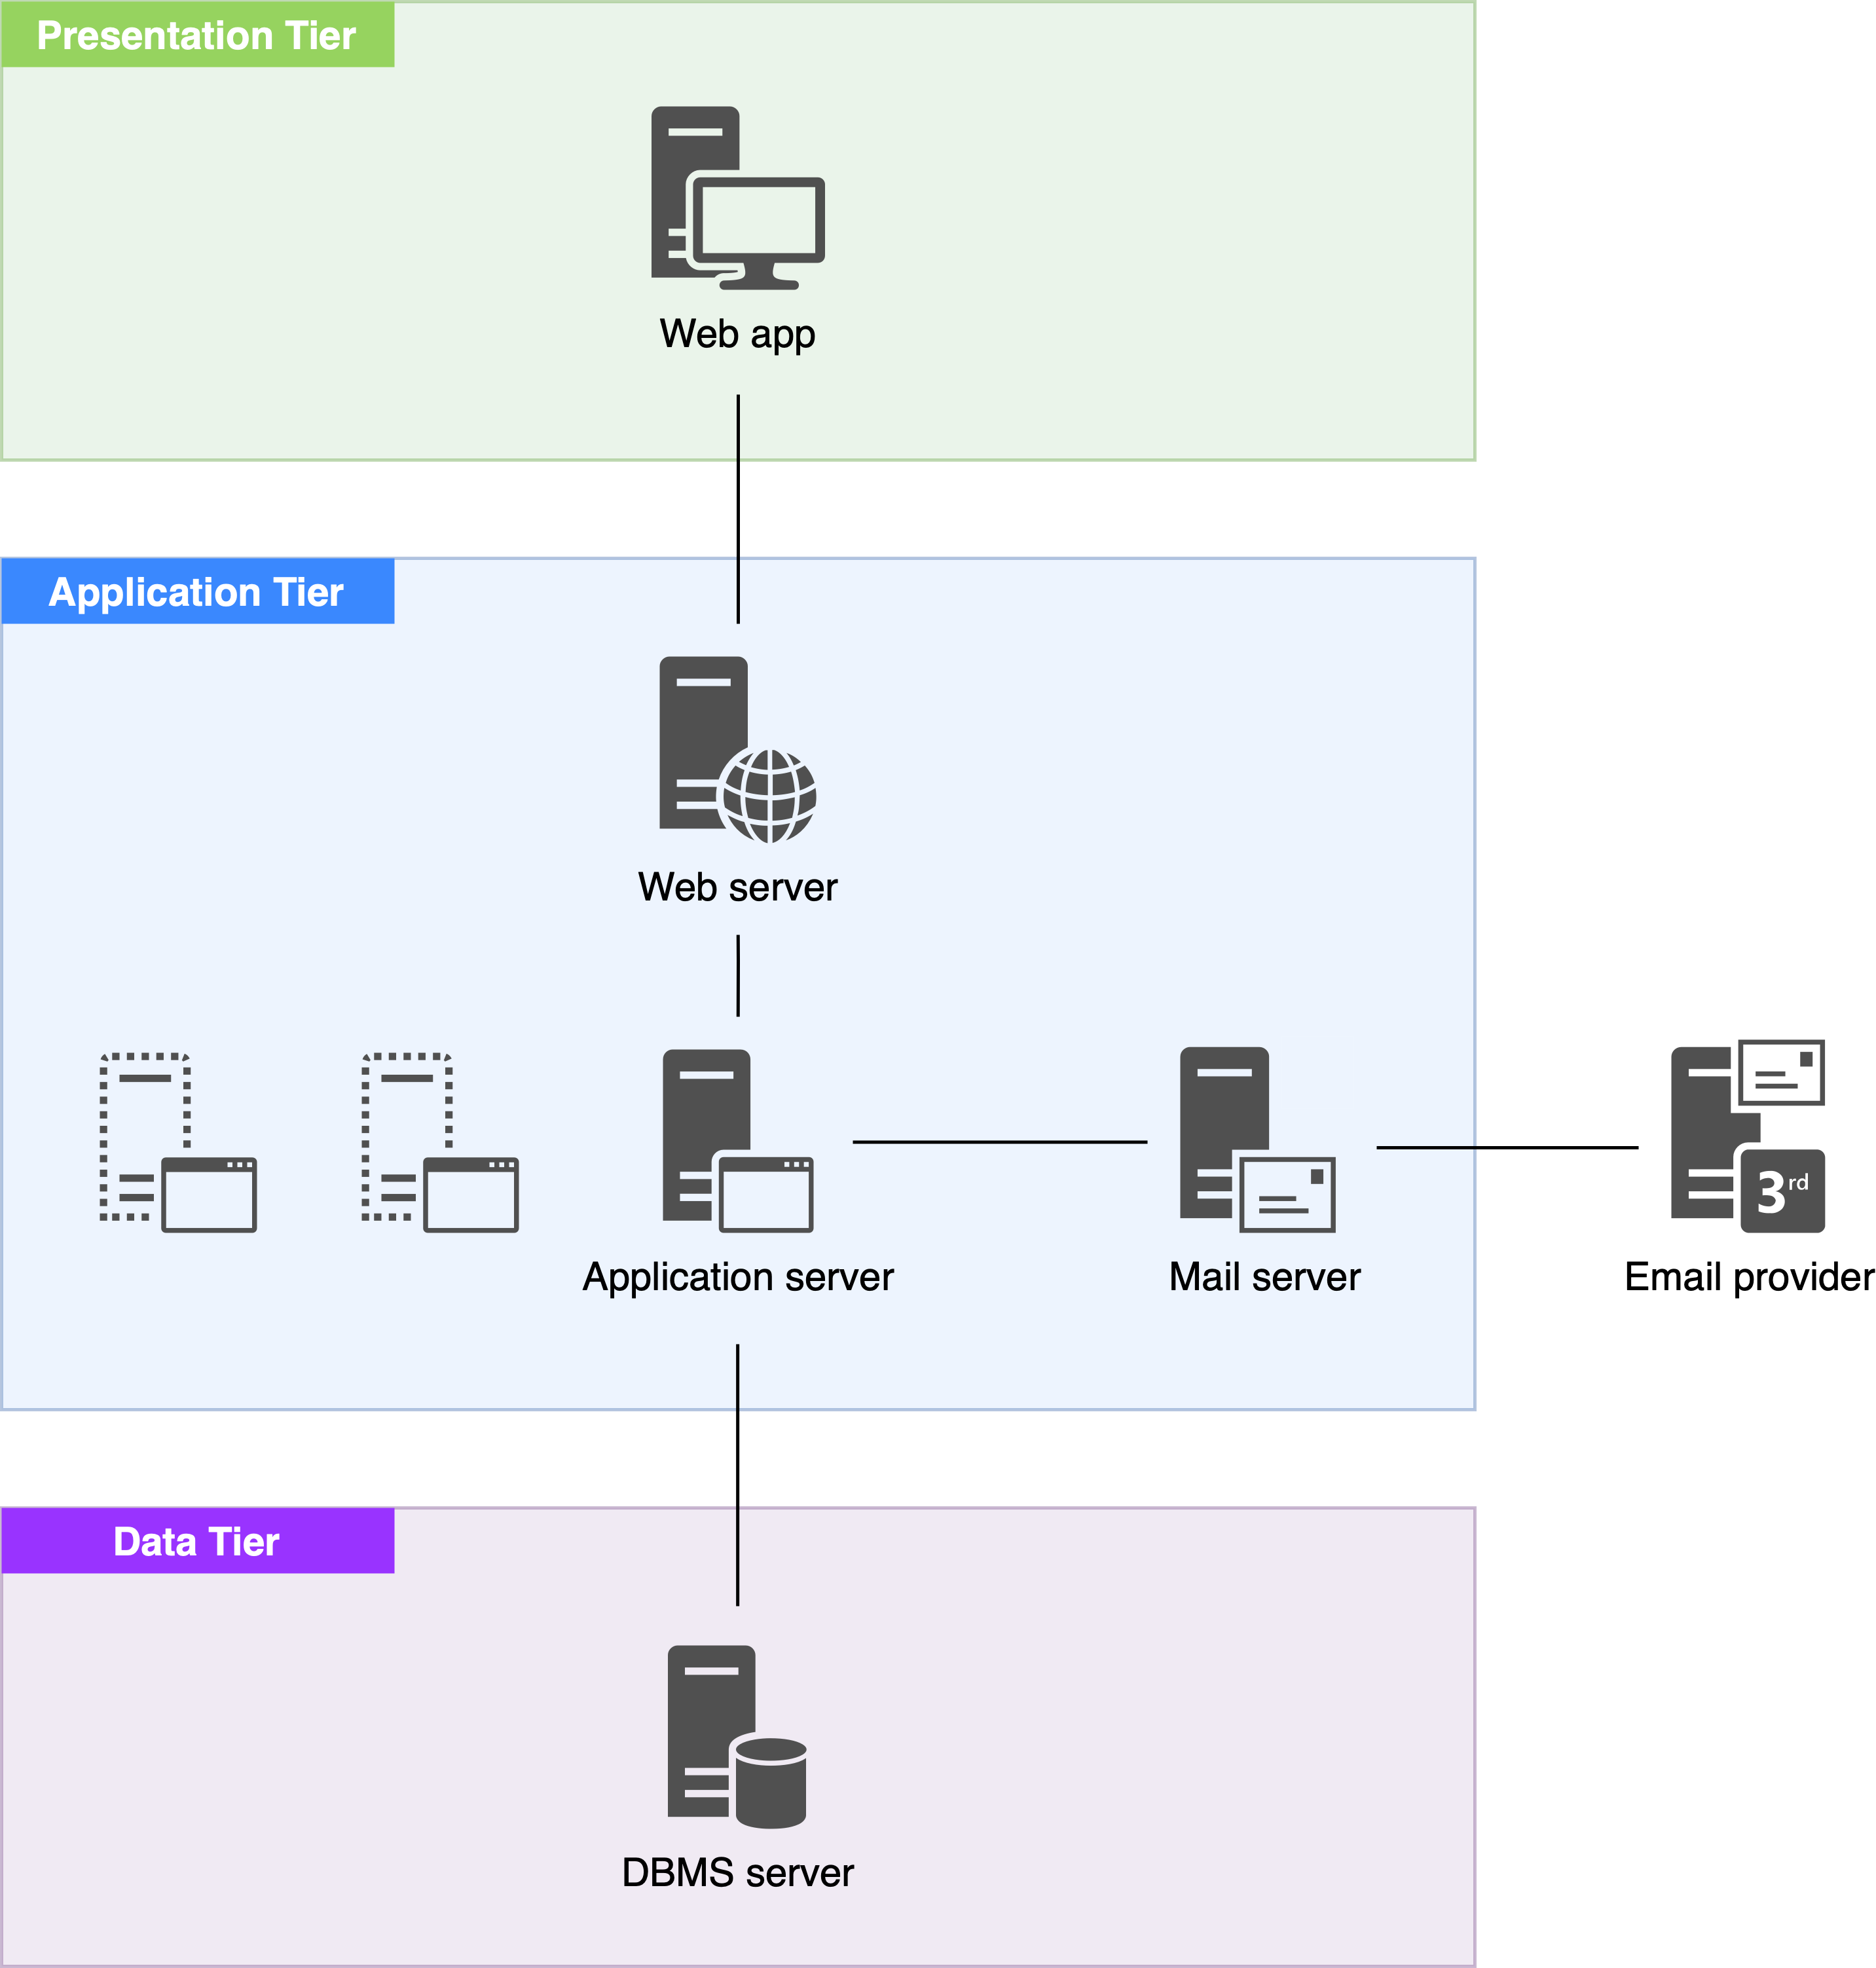
\includegraphics[width=14cm]{images/architecture.png}
    \caption{Architecture}
\end{figure}

\section{Component View}
This section illustrates the logical organization of Students\&Companies by breaking down the system into its major software modules and mapping their relationships.
Using a series of increasingly detailed UML diagrams, the component view first presents a high-level diagram showing the main system elements and their key interactions.
It then dives into individual components, examining their internal structures, responsibilities and interfaces, with particular attention to how they collaborate to implement the platform's core functionality.

\subsection{High-Level Diagram}
The high-level diagram below shows the components of Students\&Companies and their interactions.
The system exposes six distinct interfaces to the Web App, each corresponding to a manager responsible for a specific domain of functionality.

\begin{figure}[h]
    \centering
    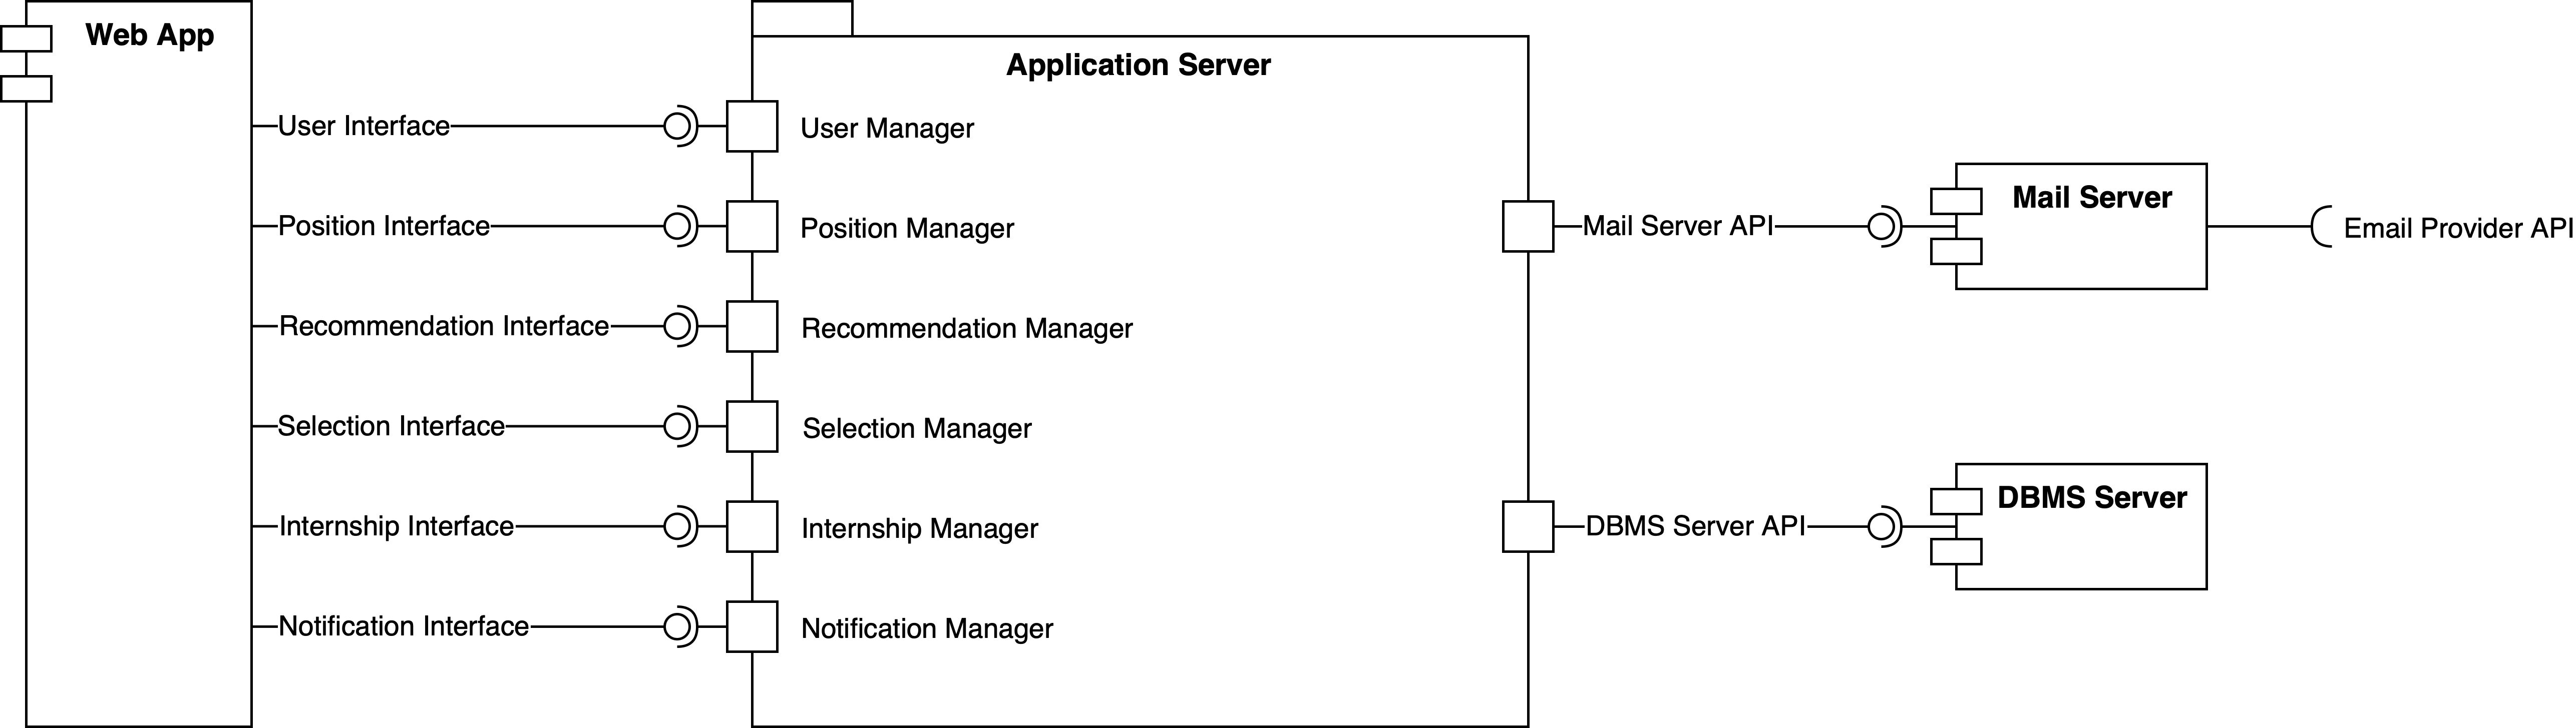
\includegraphics[width=16cm]{images/component-view/high-level.png}
    \caption{High-level component view}
\end{figure}

\subsubsection{User Manager}
The User Interface links to the User Manager, which is responsible for registration, authentication and profile management.
When users sign up, the User Manager coordinates with the Mail Server API to send confirmation emails and stores encrypted credentials through the DBMS Server API.
It also enables users to update their profiles, including uploading CVs, specifying preferences and managing account settings.

\subsubsection{Position Manager}
The Position Interface interacts with the Position Manager, enabling companies to post internship positions and students to search for them.
Companies use this interface to specify position details such as tasks, application domains, required skills, terms and additional benefits, all securely stored through the DBMS Server API.
Students can search for positions using keywords or by applying filters such as domain or location, with the manager retrieving these records from the DBMS Server API.

\subsubsection{Recommendation Manager}
The Recommendation Interface connects to the Recommendation Manager, which powers the platform's matching and recommendation capabilities.
Beyond simple keyword searches, this manager leverages statistical analysis to compare students' profiles with position descriptions, generating recommendations for both students and companies.
These recommendations are stored and retrieved through the DBMS Server API.
To facilitate communication, the Recommendation Manager uses the Mail Server API to notify students and companies about new recommendations, ensuring proactive and timely engagement with suitable matches.

\subsubsection{Selection Manager}
The Selection Interface links to the Selection Manager, which coordinates the selection workflow between companies and students.
This manager handles the creation and management of structured questionnaires submitted by companies to evaluate students, storing these forms and their responses through the DBMS Server API, and it manages the scheduling of interviews.
Throughout the selection process, this manager tracks the status of applications, logging and updating their progression in the DBMS Server.
Any changes in selection status, such as invitations for interviews or feedback from companies, are communicated to relevant parties using the Mail Server API to ensure everyone remains informed and up to date.

\subsubsection{Internship Manager}
The Internship Interface connects to the Internship Manager, which oversees all active internships.
This manager allows students, companies and universities to monitor progress, share updates, submit reports and raise concerns through a collaborative interface.
Progress reports, feedback logs and other internship data are stored and retrieved using the DBMS Server API.
When an issue or concern is raised, the manager notifies the relevant parties, including universities, through the Mail Server API, ensuring swift communication.

\subsubsection{Notification Manager}
The Notification Interface is responsible for handling asynchronous communication from the Notification Manager to users.
This manager ensures the delivery of updates, including notifications about new matches identified by the Recommendation Manager, changes in the selection process from the Selection Manager or updates on the internship progress through the Internship Manager.
Notifications are prepared by other managers and delivered to users through the Notification Manager, which uses the Mail Server API for communication.
For tracking and auditing purposes, this manager also logs all notifications into the DBMS using the DBMS Server API, ensuring a record of all communications for reference when needed.

\subsection{Low-Level Diagram}
\subsection{Managers}
\section{Deployment View}
\section{Runtime View}
\section{Component Interfaces}
\section{Architectural Styles and Patterns}
This section examines the architectural styles adopted in Students\&Companies, explaining their general principles and how they guide implementation decisions.
Understanding these foundational patterns is crucial for developers working on the system, as they influence everything from component interaction to code organization.

\subsubsection{Client-Server Architecture}
The system's foundation rests on a client-server architecture, which separates systems into service requesters, called clients, and service providers, called servers.
This separation enables the user interface to evolve independently from data processing and storage, while centralizing resource management on the server side.
Developers can thus focus on their specific domain, either crafting responsive user experiences or implementing robust server-side logic.

Modern applications refine this pattern through tiers, logical groupings of related functionality.
A three-tier architecture divides the application into three distinct layers: a presentation tier that handles the user interface, an application tier that processes business logic and a data tier that manages storage.
This separation gives developers clear boundaries for their work: interface developers can update the presentation tier without considering database queries, application developers can enhance business logic without touching the user interface and database administrators can optimize storage without impacting other tiers.
Each team works independently, reducing development bottlenecks and simplifying maintenance.

\subsubsection{REST Architecture}
REST (Representational State Transfer) guides how these tiers communicate over the web.
Originally conceived for document transfer, REST has evolved into a comprehensive style for data exchange.
Its core principle of statelessness means that servers maintain no information about past requests.
Instead, each client request must contain all necessary context.
This architectural choice significantly impacts development: backend developers need not manage complex session states, system administrators benefit from straightforward load balancing since any server can handle any request and cache developers can optimize performance by focusing solely on request parameters rather than server state.

\subsubsection{Event-Driven Architecture}
The system also employs an event-driven architecture, organizing certain components around event production and consumption rather than direct coupling.
When a company posts a new internship position, for example, the system generates an event rather than directly notifying students.
This architectural choice lets developers add new features without modifying existing code, as they simply subscribe new components to relevant events.
The pattern particularly shines in notifications and real-time updates, providing a clean separation between event producers and consumers.

\section{Other Design Decisions}
While architectural styles and patterns provide the system's foundation, many other critical design decisions shape its implementation.
This section outlines these choices, focusing on practical aspects that developers must consider when implementing the system.

\subsubsection{Deployment Approach}
The deployment strategy embraces horizontal scaling, running multiple application server instances rather than scaling up individual servers.
This approach requires developers to write stateless code that works across instances, but provides significant benefits: the system continues functioning even if some instances fail, resource allocation becomes more flexible as administrators can add or remove instances based on demand and load balancing becomes straightforward since any instance can handle any request.

\subsubsection{Security Implementation}
Security permeates every aspect of the design through multiple complementary layers.
All client-server communication uses HTTPS encryption, protecting data in transit.
Sensitive user information receives additional encryption in the database.
Session management relies on secure, time-limited authentication tokens rather than storing session data server-side.
These decisions guide security-related development work, from implementing proper token handling to ensuring sensitive data never appears in logs.

\subsubsection{Data Management}
Data management emphasizes both integrity and performance.
The database implements transaction management to maintain consistency even during concurrent operations.
Constraint enforcement at the database level catches data validity issues early.
Performance optimization through strategic indexing and caching improves response times.
These choices influence how developers interact with data, as they must properly manage transactions, respect constraints and consider query performance during development.
